%!TEX root = ./main.tex

For the rest of this document, we will use the Qi-Wu-Zhang (QWZ) model as our example for a topological insulator, first introduced in \cite{qi_topological_2006}. This is because the QWZ model is a simple toy model for a two-dimensional topological insulator with nearest-neighbour interactions on a square lattice.\par
 We work in a similar Hilbert space as that used in \textsection\ref{sec:lattice_bloch}, on a lattice of unit cells indexed by a two dimensional lattice vector $\bf m$, where each cell contains two sites -- the QWZ model has two bands. Thus the Hilbert space of the system is spanned by states of the form
\begin{align}
    \ket{\psi} = \ket{m_x} \otimes \ket{m_y} \otimes \ket{\alpha}.
\end{align}
The lattice has size $(L_x,L_y)$, so we have 
\begin{align}
    m_x \in \{ 0,...,L_x-1\}\\
    m_y \in \{ 0,...,L_y-1\}\\
    \alpha \in \{0,1\}.
\end{align}
The QWZ model is defined by three terms, a hopping between unit cells in the $x$-direction, a hopping in the $y$-direction, and a staggered on-site potential whose strength is determined by a parameter $u$.
\begin{align}
    \hat H &= \sum_{\bf m} \ket{\bf m+ 1_x}\bra{\bf m} \otimes \frac{\sigma_z + i\sigma_x}{2} + h.c. \nonumber \\
    &+ \sum_{\bf m} \ket{\bf m+ 1_y}\bra{\bf m} \otimes \frac{\sigma_z + i\sigma_y}{2} + h.c. \nonumber \\
    &+ \sum_{\bf m} \ket{\bf m}\bra{\bf m} \otimes u\; \sigma_z,
\end{align}
where $1_x$ and $1_y$ represent the unit displacement in their respective directions,
\begin{align}
	1_x = \begin{pmatrix}
	1\\
	0
	\end{pmatrix}, \ 1_y = \begin{pmatrix}
	0\\
	1
	\end{pmatrix}.
\end{align}
\begin{figure}[t]
\begin{center}
 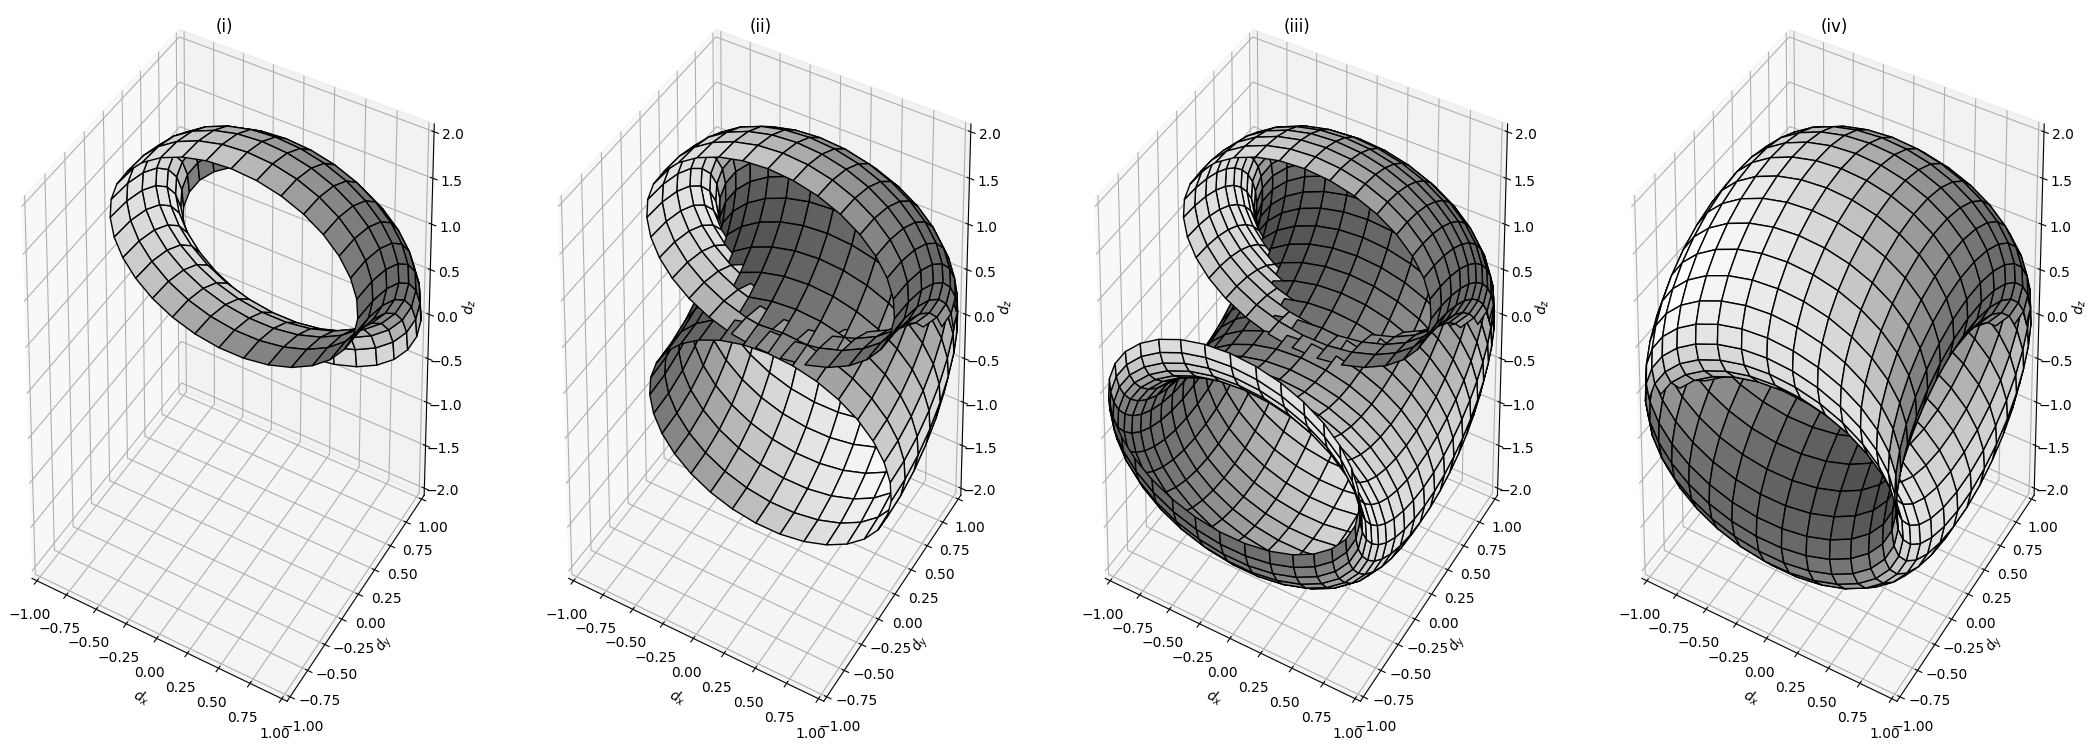
\includegraphics[width=\textwidth]{QWZ_donut}
\caption{The embedding of the Brillouin zone in $\bf d$-space for the QWZ model. This is shown in four progressive cutaways to ensure the internal structure can be seen. In all four images $k_x$ spans the interval $\left ( 0, 2\pi \right ]$, however in (i) $k_y$ spans $\left ( 0, \frac{\pi}{2} \right ]$, in (ii) $k_y$ spans $\left ( 0, \pi \right ]$, in (iii) $k_y$ spans $\left ( 0, \frac{3 \pi}{2} \right ]$, and in (iv) $k_y$ spans $\left ( 0, 2\pi \right ]$. }
\label{fig:QWZ_donut}
\end{center}
\end{figure}
Using Bloch's theorem, we can find the bulk Hamiltonian,
\begin{align}
    \hat H(\bf k) = \begin{pmatrix}
\sin k_x \\ 
\sin k_y\\ 
u + \cos k_x+ \cos k_y
\end{pmatrix} \cdot \bm \sigma.
\end{align}
Here, $k_x$ and $k_y$ determine our position in the Brillouin zone. As explained in \textsection\ref{sec:an_example}, this represents the embedding of a torus in $\bf d$-space, shown in fig. \ref{fig:QWZ_donut}.\par
The $u$-parameter has the effect of translating the torus by a fixed amount in the $z$-direction. From this we can see that the QWZ model only has non-zero Chern number for values of $u$ between -2 and 2. This is because translating the torus by any more than this will place the origin completely outside. The Chern number for the QWZ model is
\begin{align}
Q = \left\{\begin{matrix}
-1 &:&  -2 < u < 0 \\ 
1  &:&  0<u<2\\
0  &:&  \textit{otherwise} 
\end{matrix}\right. ,
\end{align}
not including the points at $u =$ -2, 0 and 2, at which the Chern number is undefined because the band gap closes and the material is conducting. Some example band structures for varying values of $u$ are shown in fig. \ref{fig:QWZ_band_struct}.
\begin{figure}[t]
\begin{center}
 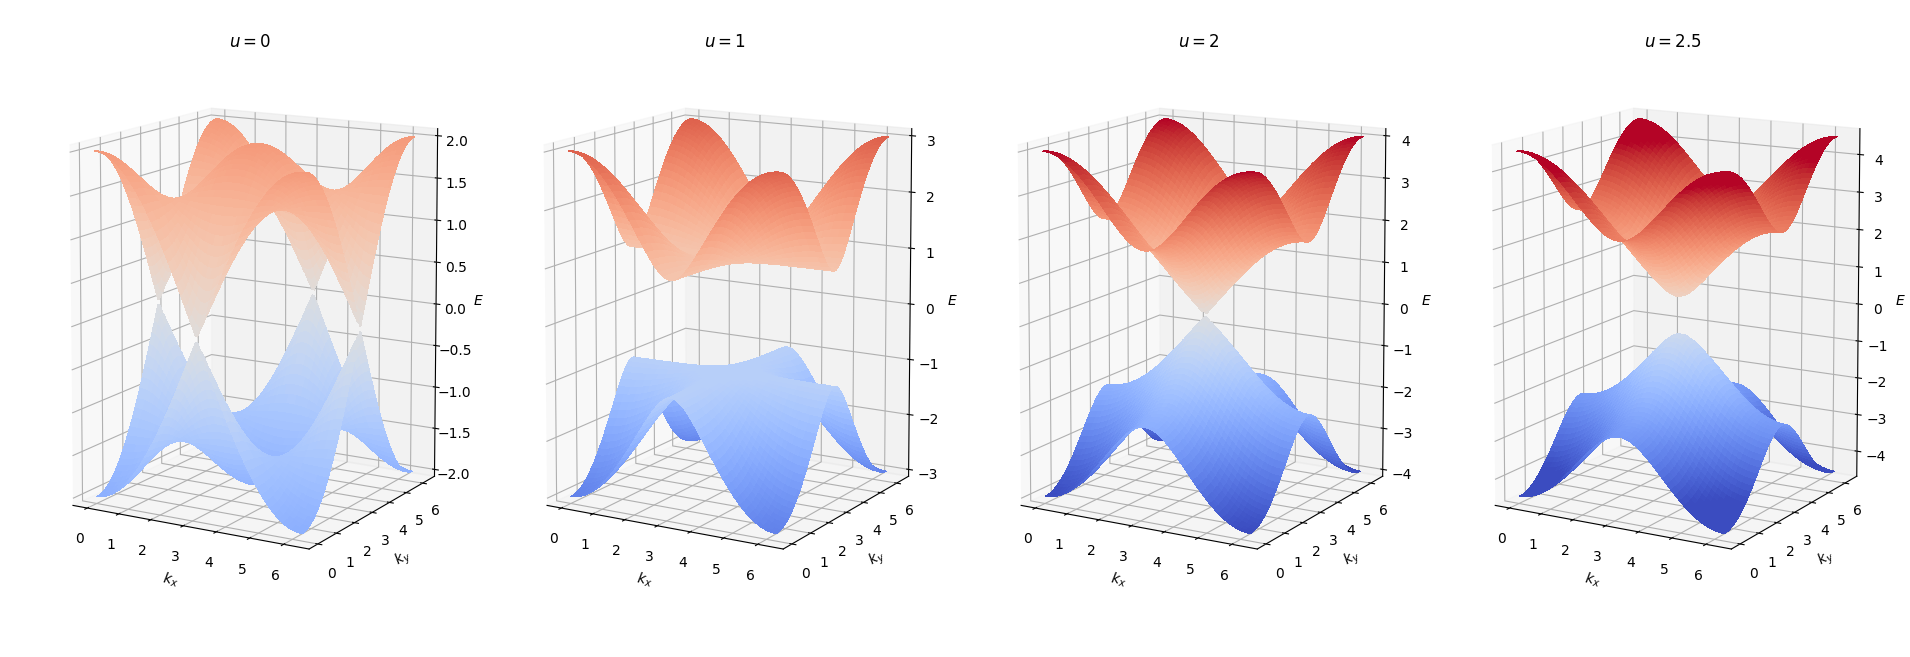
\includegraphics[width=\textwidth]{QWZ_band_struct}
\caption{Four examples of the band structure of the QWZ model are shown, for varying $u$ values between 0 and 2.5. At $u$ = 0 and 2, the bands touch and Chern number is undefined. At $u$ = 1, Q = +1, and at $u$ = 2.5, Q = 0.}
\label{fig:QWZ_band_struct}
\end{center}
\end{figure}

\subsection{Strip Geometry} \label{sec:QWZ_strip_geometry}
In much of the following discussion, we will be studying the QWZ model in a system with strip geometry. This means that the lattice is periodic and uniform in the $y$-direction, but is allowed to be non-uniform or have open boundaries in the $x$-direction. We will allow $u$ to vary in the $x$-direction, so add a subscript to indicate position-dependence $u \rightarrow u_{m_x}$. We can apply Bloch's theorem in the $y$-direction only, and our eigenstates take the following form,
\begin{align}
    \ket{\psi} = \ket{k_y}\otimes \ket{v_{k_y}^{n,l}},
\end{align}
where $\ket{k_y}$ is a plane wave solution
\begin{align}
    \ket{k_y} =\frac{1}{\sqrt{L_y}} \sum_{m_y} e^{i m_y k_y}\ket{m_y},
\end{align}
and $\ket{v_{k_y}^{n,l}}$ is a $2L_x$-element vector in the remaining part of the Hilbert space $\mathcal H_x \otimes \mathcal H_{\textup{int}} $. The $n$ index labels which band the state is in, and the $l$ index differentiates between the states in each band.
\begin{align}
    n &\in \{0,1\}\\
    l &\in \{ 0, \dots ,L_x -1\}.
\end{align}
The $v$-states are solutions of the semi-bulk Hamiltonian
\begin{align}
    \hat H(k_y) &= \sum_{m_x} \ket{m_x+1}\bra{m_x} \otimes \frac{\sigma_z + i\sigma_x}{2} + h.c.\nonumber \\
    &+ \sum_{m_x} \ket{m_x}\bra{m_x} \otimes \left [ (u_{m_x} + \cos k_y) \; \sigma_z + \sin k_y \; \sigma_y  \right ].
\end{align}
We have effectively reduced our system from a lattice of interacting sites in $x$ and $y$, to a set of chain models in $x$, that are each labelled by a value of $k_y$.
\begin{center}
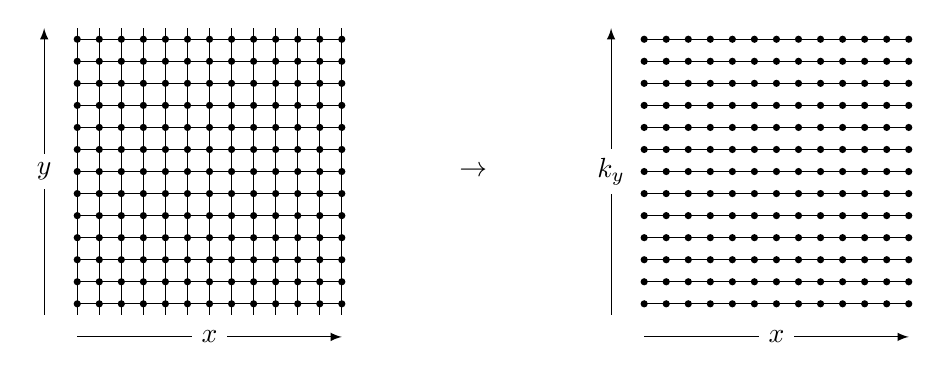
\begin{tikzpicture}

\def \cellsize{0.28}
\def \numcells{6}
\def \pos {3.6}

\foreach \x in {-\numcells, ..., \numcells}{
\draw [] (\x*\cellsize - \pos, -\numcells*\cellsize -0.5*\cellsize) -- (\x*\cellsize - \pos, \numcells*\cellsize + 0.5*\cellsize);
}
\foreach \y in {-\numcells, ..., \numcells}{
\draw [] (-\numcells*\cellsize -\pos, \y*\cellsize) -- (\numcells*\cellsize - \pos, \y*\cellsize);
} 

\foreach \x in {-\numcells, ..., \numcells}{
\foreach \y in {-\numcells, ..., \numcells}{
\fill[] (\x*\cellsize - \pos, \y*\cellsize) circle (1.3pt);
}
}

\draw [-latex] (-\numcells*\cellsize -\pos, -\numcells*\cellsize - 1.5*\cellsize) -- (\numcells*\cellsize - \pos, -\numcells*\cellsize - 1.5*\cellsize);
\draw node [fill= white] at (-\pos, -\numcells*\cellsize - 1.5*\cellsize) {$x$};

\draw [-latex] (-\numcells*\cellsize - 1.5*\cellsize - \pos, -\numcells*\cellsize -0.5*\cellsize) -- (-\numcells*\cellsize - 1.5*\cellsize - \pos, \numcells*\cellsize + 0.5*\cellsize);
\draw node [fill= white] at  (-\numcells*\cellsize - 1.5*\cellsize - \pos, 0) {$y$};

\draw node at (-0.25,0) {$\huge \rightarrow$};


\foreach \y in {-\numcells, ..., \numcells}{
\draw [] (-\numcells*\cellsize +\pos, \y*\cellsize) -- (\numcells*\cellsize + \pos, \y*\cellsize);
} 

\foreach \x in {-\numcells, ..., \numcells}{
\foreach \y in {-\numcells, ..., \numcells}{
\fill[] (\x*\cellsize + \pos, \y*\cellsize) circle (1.3pt);
}
}

\draw [-latex] (-\numcells*\cellsize +\pos, -\numcells*\cellsize - 1.5*\cellsize) -- (\numcells*\cellsize + \pos, -\numcells*\cellsize - 1.5*\cellsize);
\draw node [fill= white] at (+\pos, -\numcells*\cellsize - 1.5*\cellsize) {$x$};

\draw [-latex] (-\numcells*\cellsize - 1.5*\cellsize + \pos, -\numcells*\cellsize -0.5*\cellsize) -- (-\numcells*\cellsize - 1.5*\cellsize+ \pos, \numcells*\cellsize + 0.5*\cellsize);
\draw node [fill= white] at  (-\numcells*\cellsize - 1.5*\cellsize + \pos, 0) {$k_y$};

\end{tikzpicture}
\end{center}
We can rewrite this, in terms of the $2\times2$ matrices $A$ and $B$,
\begin{align}
    A &= (u + \cos k_y) \; \sigma_z + \sin k_y \; \sigma_y,  \\ 
    B &= \frac{\sigma_z + i\sigma_x}{2},
\end{align}
and express our wavevectors in terms of a set of $L_x$ two-element states $\psi_n$
\begin{align}
    \ket{\psi} = \begin{pmatrix}
    \psi_0 \\
    \psi_1 \\
    \vdots \\
    \psi_{L_x -1}
     \end{pmatrix},
\end{align}
to arrive at a set of equations for the eigenvalues of the semi-bulk Hamiltonian.
\begin{align}
    \textup{Bulk:} &\ A\psi_n + B\psi_{n+1} + B^\dag \psi_{n-1} = \lambda \psi_n \\
    \textup{Left Edge:} &\ A\psi_1 + B\psi_{2} = \lambda \psi_1\\
    \textup{Right Edge:} &\ A\psi_{L_x} + B^\dag \psi_{L_x-1}  = \lambda \psi_n
\end{align}
The band structure for this system in both periodic boundaries and strip geometry is shown in fig. \ref{fig:strip_energy}.
\begin{figure}[t]
\begin{center}
 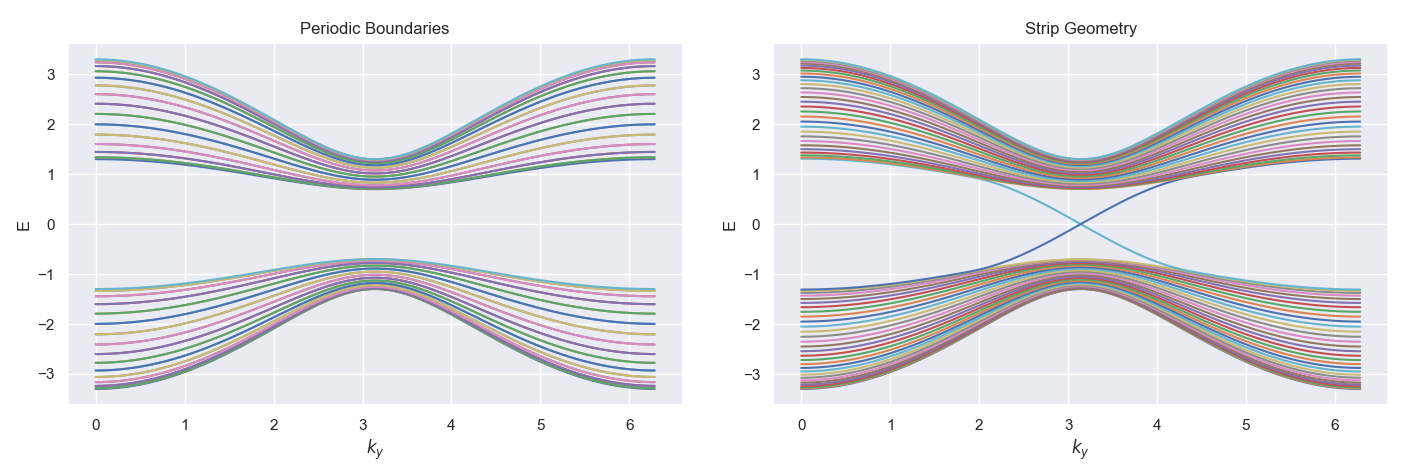
\includegraphics[width=.85\textwidth]{strip_energy}
\caption{An example band structure for a QWZ model with $u$ = 1.3 and $L_x$ = 30. On the left is the example for periodic boundary conditions, showing two well-separated bands. On the right is the case for open boundary conditions. Two edge states are shown leaving the bulk and crossing the gap, with the descending state being a left edge state, and the ascending state being a right edge state. }
\label{fig:strip_energy}
\end{center}
\end{figure}
We can now look at solving this analytically for the bulk and edge states. We will omit this calculation and print only the form of the results, however a full derivation can be found in appendix \ref{sec:QWZ_model_appendix}. Note that edge states are only present for certain values of $k_y$, which can be seen in figure \ref{fig:strip_energy}, where the edge states only separate from the bulk in a region around $k_y = \pi$. \par
Edge states have the form
\begin{align}
    \ket{\psi^{\textup{left}}_{k_y}} = \sqrt{1-\xi_l^2}\sum_{m=1}^{L_x} \xi_l^{m-1}\ket m \otimes \begin{pmatrix}
    1\\
    -i
    \end{pmatrix}
\end{align}
where 
\begin{align}
    \xi_l &= -u - \cos k_y.
\end{align}
This state has energy
\begin{align}
    E_l &= -\sin k_y.
\end{align}
Similarly, the right edge state is given by
\begin{align}
    \ket {\psi^{\textup{right}}_{k_y}} = \sqrt{1-\xi_r^2} \sum_{m=1}^{L_x} \xi_r^{L_x-m} \ket m \otimes  \begin{pmatrix}
    1\\
    i
    \end{pmatrix}
\end{align}
with the extra conditions
\begin{align}
   	 \xi_r &= -u-\cos k \label{eqn:edge_condition}\\
	E_r &= \sin k.
\end{align}
These edge states are only valid solutions for $k_y$ in the region
\begin{align}
	-1 < u+\cos k_y < 1.
\end{align}
These limits can be seen in fig. \ref{fig:strip_energy}, where the edge states peel away from the bands to cross the energy gap.\par
The bulk states are less straightforward to obtain exact solutions for, we give the general form for them and leave the details to appendix \ref{sec:QWZ_model_appendix}.
\begin{align}
    \ket{\psi^\pm_{k_y} }= \frac{1}{\sqrt{L_x}}\sum \ket{m}  \otimes \left [ \alpha e^{i \theta m} \ket{\phi_{\theta}^{\pm}} + \beta e^{-i \theta m} \ket{\phi_{\theta}^{\pm *}} \right ],
\end{align}
where the exact values of $\theta$, $\alpha$, $\beta$ and $\ket{\phi_{\theta}^{\pm}} $ can be found by solving some fairly unpleasant equations.\par
Here we mention a final caveat, These calculations are only strictly valid in the limit of a large system. This is because we have made the assumption the edge states can be calculated by taking into consideration only one edge and ignoring the effect of the other. The edge states decay exponentially through the system, so we are relying on the assumption that the edge state has effectively decayed to nothing before reaching the other side. When this condition is relaxed the edge states are able to couple to one another. This has a two effects, the first being that at the crossing of edge states, our energy eigenvalues become positive and negative superposition states of both edge states. The other is that the left state coupling to the right state shifts their energy levels such that no states cross $E = 0$ -- there is no longer a crossing of energy levels for the left and right edge states.






